%% Jason Chalom 711985 Honours 2017

\documentclass [11pt]{article}
\usepackage{titlesec}
\usepackage{hyperref}
\usepackage{graphicx}
\usepackage[normalem]{ulem}
\useunder{\uline}{\ul}{}
\usepackage{float}
\usepackage{enumitem}
\usepackage[title,titletoc,toc]{appendix}
\usepackage{geometry}
\geometry{
	a4paper,
	total={170mm,257mm},
	left=20mm,
	top=20mm,
}

\graphicspath{ {images/} }

\title{Research Proposal\\\medskip An Investigation of AI Tree Search Methods and Their Effectiveness at Playing the Card Game Gwent\\\medskip}
\author{Jason Chalom (711985)\\Supervisor: Professor Clint Van Alten\\\\University of the Witwatersrand\\School of Computer Science and Applied Mathematics}

\titleclass{\subsubsubsection}{straight}[\subsection]

\newcounter{subsubsubsection}[subsubsection]
\renewcommand\thesubsubsubsection{\thesubsubsection.\arabic{subsubsubsection}}
\renewcommand\theparagraph{\thesubsubsubsection.\arabic{paragraph}} % optional; useful if paragraphs are to be numbered

\titleformat{\subsubsubsection}
{\normalfont\normalsize\bfseries}{\thesubsubsubsection}{1em}{}
\titlespacing*{\subsubsubsection}
{0pt}{3.25ex plus 1ex minus .2ex}{1.5ex plus .2ex}

\makeatletter
\renewcommand\paragraph{\@startsection{paragraph}{5}{\z@}%
	{3.25ex \@plus1ex \@minus.2ex}%
	{-1em}%
	{\normalfont\normalsize\bfseries}}
\renewcommand\subparagraph{\@startsection{subparagraph}{6}{\parindent}%
	{3.25ex \@plus1ex \@minus .2ex}%
	{-1em}%
	{\normalfont\normalsize\bfseries}}
\def\toclevel@subsubsubsection{4}
\def\toclevel@paragraph{5}
\def\toclevel@paragraph{6}
\def\l@subsubsubsection{\@dottedtocline{4}{7em}{4em}}
\def\l@paragraph{\@dottedtocline{5}{10em}{5em}}
\def\l@subparagraph{\@dottedtocline{6}{14em}{6em}}
\makeatother

\setcounter{secnumdepth}{4}
\setcounter{tocdepth}{4}

\newenvironment{myitemize}
{ \begin{itemize}
		\setlength{\itemsep}{0pt}
		\setlength{\parskip}{0pt}
		\setlength{\parsep}{0pt}     }
	{ \end{itemize}                  } 

\newcommand{\itab}[1]{\hspace{0em}\rlap{#1}}
\newcommand{\tab}[1]{\hspace{.2\textwidth}\rlap{#1}}

\begin{document}
	\maketitle
	\vfill
	
	\break
	
	\tableofcontents
	\break
	
	\section*{Abstract}
	%10 lines
	The aim of this research is to compare Monte-Carlo tree search and minimax methods applied to the game Gwent and then build a hybrid method. This method incorporates both types of tree searches in an attempt to produce an AI which provides the benefits of both approaches. Gwent is an interesting domain because it is non-deterministic and has sub-domains which require their own search operations to be performed when decisions are made which incorporate those sub-domains. The experimental framework will be implemented in C++. The algorithms will be analysed by using AI-versus-AI simulations in a tournament style setup.
	
	\section{Introduction}
	The textbook, Artificial Intelligence: A Modern Approach \cite{AIModern} describes games as having been an area of interest for humans since the beginning of organised societies. A game is where two players or agents are in competition in some domain with a defined set of rules. Research in artificial intelligence (AI) has always gravitated towards games due to the complexity and abstractedness they present and yet they have clearly defined rules which make them easier to program and study than other abstract real-world problems such as physical sport. The applications of AI in games can lead to developments in other more serious fields such as applications in economics. \\
	
	\noindent Not all games are the same. Artificial Intelligence: A Modern Approach \cite{AIModern} describes many games such as deterministic games where the outcomes are known, turn based games where each player must wait their turn, two-player games and zero-sum games where in a multi-player arena only one player can win as whatever gains (wins) one player gets the other player must then lose out on. A game with perfect information means that both players know full-well what the outcomes of all previous moves were. \\
	
	\noindent Games are an interesting area of study because of how difficult they can be. Many games are computationally difficult to solve - both in complexity and time. Some games can have so many states that would have to be computed that it is infeasible to calculate all of them within the time constraints of a game where inefficiency could have penalties. Also due to the very nature of deriving game decisions and paths for future moves, having branching factors which depend on the types of games being solved will produce exceedingly large solution spaces. This means that strategies which employ smart use of resource constraints in a given domain are required to solve these problems. \cite{AIModern}. \\
	
	\subsection{Problem Domain: The Card Game Gwent}
	The Gwent game guide \cite{guide} describes Gwent as a two-player turn-based card game based on a medieval, fantasy battle field. It is a game played to the best of three rounds where the players use the same hand of cards drawn from their respective shuffled decks prior to start of play. Each player creates a deck from the total cards they have based on a certain faction and they choose cards whilst following a set of rules which govern how theses decks should be constructed. There are a few different rule sets and as new cards are introduced to the game new rules may be added. This game is interesting because it is a zero-sum game with partial information. The players both know the moves which came before but they do not know the opposing players hand, or even what cards are in their decks. Gwent has a number of interesting rules such as there being a card which allows a player to select a card from their discard pile and playing it again. Another interesting card is one which the player plays on the opposing side of the board. Here the card acts against the player who played the card in return for two new cards from the player’s deck.
	
	\subsection{Aim of Research}
	Gwent is an unknown domain in terms of how different variants of tree search algorithms such a hybrid of MCTS and minimax may perform. A search through existing literature has not found any research which applies these methods to this exact problem. Gwent is also a relatively new game which has only been out for the last two years which may explain the lack of its use in existing literature. This investigation will be done by doing experimental analysis of the aforementioned algorithms and analysing the results that will be generated. 
	
	\subsection{Expected Results}
	The expected outcome of this investigation is that of the algorithms tested, a hybrid of Monte-Carlo Tree Search and minimax will be more accurate and faster than the standalone methods. All the tree search algorithms investigated are expected to perform better than a random agent.
	
	\subsection{Structure of Proposal}
	In this proposal I will be reviewing related research in the field of artificial intelligence such as different techniques that can be used to improve the performance of tree search algorithms and also different tree search algorithms. I will look at different testing methodologies used by other researchers when dealing with these kinds of problem domains. 
	The hypothesis for this research is stated with an accompanying motivation. A detailed description of the proposed methodology and a related plan to complete this study within the remainder of the academic year. The research plan describes in detail the risks of this proposed project, what deliverables are required, the criteria that can be used to measure the success of the research, its outcomes and a breakdown of the time and how it will be used. This document will then conclude by arguing why this research should be conducted.
	
	\subsection{Conclusion}
	AI, games and algorithm research is both fascinating and important for future progress in not only making computing systems better adversaries for playing games but also for improving their capabilities to help humans in making decisions in other related domains which have more practical and potentially more serious uses. My proposed research hopes to apply established AI search algorithms on a new game domain with the expectation of showing that a hybrid method will be the best performing of the tested algorithms. The background \ref{background} will expand on the problem domain and provide details on current AI tree search research.
	
	\section{Background and Related Research}
	\label{background}
	\subsection{Introduction}
	There are many documented and analysed strategies for solving these kinds of adversarial game problems. The focus for this project is on the methods which utilize a decision tree approach to search for an optimal decision to make during play. Chapter 5 of Artificial Intelligence: A Modern Approach \cite{AIModern} deals exclusively with tree search techniques in solving adversarial game problems.
	
	\subsection{The Rules of Gwent}
	Gwent is a 2-player turn-based game, with three rounds \cite{guide}. The game is the best of three rounds. Each player must have a chosen deck which consists one leader card, twenty-two unit cards minimum, and ten special cards maximum. Unit cards which are hero cards, cannot be revived or effected by any other card. Ten random cards from the chosen deck are drawn at the start of the three rounds for both players. Each player takes a turn placing one card on the board. The board has three rows on both sides. Certain units can only be placed on certain rows. A player can also at any turn decide to pass the remainder of the round. The winner of a round is decided when either both players run out of cards, both players pass the round or a combination of the two. A round win is calculated by adding up the strength of all unit cards whilst taking into account the effects of the special cards.
	\\\\\\
	\noindent \textbf{Special Cards:}
	
	\begin{itemize}
		\item There are four types of weather cards, one clear and one for each row of the battlefield (on both sides). The weather cards reduce all unit cards except hero cards to attack points equal to one (unless commanders horn is in effect then attack points of two).
		\item The commander's horn doubles attack points of all normal unit cards in that row.
		\item Scorch destroys the strongest valued cards on the board (i.e. the highest number, any card with that number is discarded)
		\item Decoy allows a player to take a card back into their hand.
	\end{itemize}
	
	\noindent \textbf{Abilities of Some Unit Cards}:
	\begin{itemize}
		\item Spy units go to the other player’s side in return for drawing two new cards from the player's deck into their hand.
		\item Medic allows you to look through the player's discard pile and revive one unit card (must not be a special or hero card).
		\item Tight bond doubles the attack points of a group of cards of the same type of unit (with this ability) when they are placed next to one another (The doubling is calculated on the combined strength of every card in the group).
	\end{itemize}
	
	\subsection{Literature Review}
	\subsubsection{AI Tree Searches}
	The basic idea of using tree searches to make decisions in game problems is to model the problem (or domain) as a set of decisions which are in the form of a tree. Each node of the tree as described by Artificial Intelligence: A Modern Approach \cite{AIModern} are specific game states and each edge of the tree is a certain decision or a certain path which can be taken from the parent node to get to the children nodes or the next set of possible game states. The root of the tree is either the current state of the game or the initial state depending on the implementation of tree search. A terminal node on a tree is a node where either the game has reached a stop (or end) state such that no further children can be created or a limiting condition has been met which limits the depth of the tree.
	
	\subsubsection{Tree Pruning}
	One notable problem with the approach of generating trees based on possible domain states of a game is the sheer size and complexity which can emerge from many games such as Gwent and its contemporaries. Edwards et al. \cite{AIM030} and in chapter 5 of Artificial Intelligence: A Modern Approach \cite{AIModern} both describe how a tree constructed from all possible game states is wasteful as there are many branches which need not be considered. The growth of these trees are exponential in nature (based on the size of the domain being modelled and searched) which creates a problem of time and complexity when dealing with the implementation of such an AI. In such cases these paths can be removed from the tree because they have no effect on the outcome of the tree search. This can greatly reduce the size of the tree before a complete search is done. \\
	
	\noindent Another approach as described by Chaslot et al. \cite{progressive} is to only invalidate a node (and therefore the rest of the path that follows) which is determined to be unreliable (or as a node not visited often in a tree search) and then these nodes can be re-evaluated and selected later (based on the search algorithm utilised).
	
	\subsubsection{Minimax Algorithm}
	Having created a tree of possible paths and game states an algorithm is needed to help determine which is the most optimal path for the AI to take in order to maximize its chances of winning the game (thereby minimize the chances of the other player from winning). This sets up the AI player as the MAX player and the opponent as the MIN player. One of these algorithms is called The Minimax Algorithm. Artificial Intelligence: A Modern Approach \cite{AIModern} describes this algorithm as a method of finding an optimal set of strategies. This is done by placing a value on each node of the tree which is called the minimax value. This value is a numerical representation of how useful that decision is for the MAX Player i.e. the MAX player favours a higher value and the MIN player favours a lower value. In this set-up, for each decision that MAX makes, MIN must also make a decision and these two decisions together make-up one move on the tree - this is the basis of a multi-player game. These "half-moves" are defined by Artificial Intelligence: A Modern Approach \cite{AIModern} as a ply. The minimax decision is the decision which leads to the optimal outcome for MAX from the root node. This algorithm will recursively generate the minimax values for every child node in the tree by using an objective function which determines the numerical outcome of that specific node. Then the algorithm backpropogates up the tree updating the minimax value of the parent nodes until root is reached where it terminates. \\
	\\
	\begin{figure}[H]
		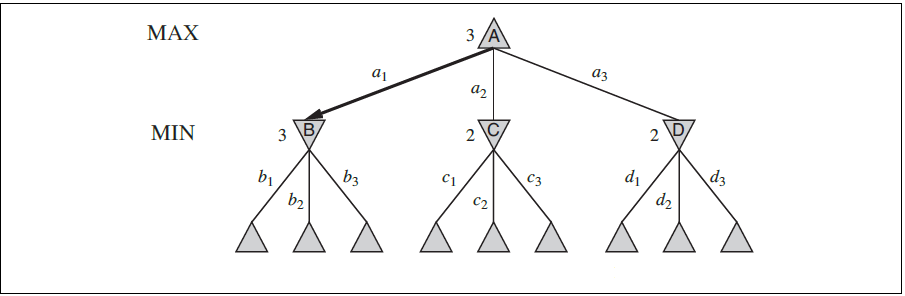
\includegraphics[width=\textwidth]{minimax}\\
		\centering
		\caption{Example of a Max tree where the Max nodes are the upright triangles and the Min nodes are down facing triangles, taken from Chapter 5 of Artificial Intelligence: A Modern Approach \cite{AIModern}.}
		\label{ab}
	\end{figure}
	
	\noindent One note which is made by Artificial Intelligence: A Modern Approach \cite{AIModern} on this algorithm is that there is an inherent assumption that both MAX and MIN play optimally. Also the Minimax algorithm in its most basic form will perform a full depth-first search of the tree which means that it will have an exponential growth in time complexity which corresponds to the exponential growth of the tree based on the domain space. The space complexity of this algorithm and the time complexity are determined by the depth of the tree and number of moves at each layer of the tree.
	
	\subsubsection{Alpha-Beta Pruning}
	The Alpha-Beta Pruning Heuristic was conceived as an extension of the minimax algorithm. Edwards et al. \cite{AIM030} states that it uses partial information from the tree to decide which branches on the tree are no longer needed for Minimax. These removed branches do not affect the final decision determined by Minimax. The method uses the fact that if a move is found to be worse than a move evaluated previously (either for the MIN player or the MAX player), than that move does not affect the outcome of the search. Edwards et al. \cite{AIM030} highlights the importance of the ordering of the possible set of plies from the current node (position) because this heuristic achieves the best results when the optimal decision is located at the beginning of the set of positions. To this effect the Alpha-Beta Heuristic can at most cut a search trees growth rate in half, which implies that this heuristic allows a computing system to search twice the depth within the same time complexity of the basic minimax algorithm. Edwards et al. \cite{AIM030} proves this by induction in their technical memo. This performance increase is a powerful first step in using Minimax in a real world domain.
	\\
	\begin{figure}[H]
		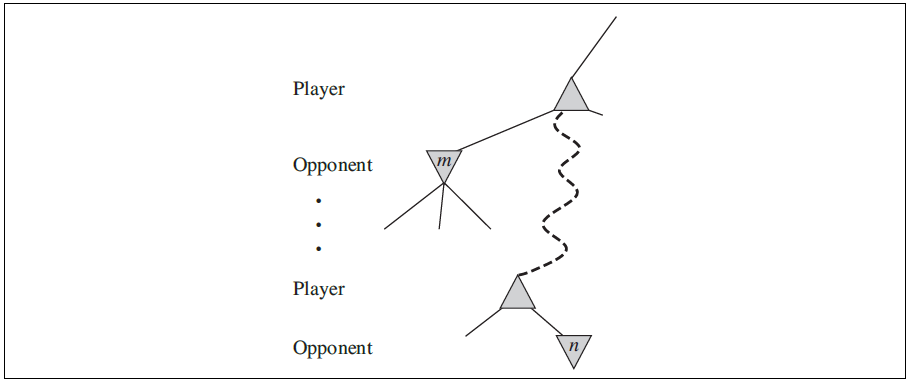
\includegraphics[width=\textwidth]{ab}\\
		\centering
		\caption{General case of alpha-beta pruning where if m is a better move than n, n will be removed, taken from Chapter 5 of Artificial Intelligence: A Modern Approach \cite{AIModern}.}
		\label{ab}
	\end{figure}
	
	\subsubsection{Other Modifications to Minimax}
	Chapter 5 of Artificial Intelligence: A Modern Approach \cite{AIModern} provides several other heuristics that can be applied to Minimax in order to deal with the exponential growth issue. These include having a cut-off condition which will only generate a tree up to a certain depth in order to contain the tree for use with computing systems which have inherent limitations. The games themselves may have limitations such as the amount of time available for making a decision. Another strategy which may be able to improve the effectiveness of Minimax in domains which are stochastic in nature and may only have partially observable information is by using Monte-Carlo simulations to generate probable states where the information is not certain. A third idea that was presented is to create a look-up table and store a set of known polices (or game heuristics) such as end states and killer moves which have proven to be effective in the past (or come from expert knowledge) and then use the look-up table when needed to make these specific decisions instead of running through a lengthy search. Such searches may then use approximations of moves past a certain depth in the tree as described by Chaslot et al. \cite{progressive} to determine most moves but retain the optimal pre-computed moves which such approximations may not choose due to the introduced error of the approximation.
	
	\subsubsection{Monte-Carlo Tree Search Algorithm}
	The basic idea of MCTS as described by James et al. \cite{wits} and Browne et al. \cite{survey} is that it combines the idea of a tree search with the idea of simulating parts of the domain space. Monte Carlo simulations are used to make approximations of some problem based on random sampling of the problem domain \cite{survey}. Browne et al. \cite{survey} describes MCTS as a family of heuristic optimisation methods for making optimal decisions in certain domains and game spaces. The basic operation of these methods sample the domain space (in similar fashion to MC methods) by simulation which is then used to build a search tree based on this sample of the domain. These methods work well with difficult problems such as hidden domains and problems where other techniques have been unsuccessful since they are stochastic in nature.\\
	
	\noindent Browne et al. \cite{survey}, James et al. \cite{wits} and Chaslot et al. \cite{progressive} all describe a basic construction of a MCTS as having four major steps: Selection, Expansion, Simulation (also known as roll-outs \cite{wits}) and Back-propagation The selection step is when the tree is traversed from the root node through to the most urgent terminating nodes of the tree - which is decided by some predefined policy. Chaslot et al. \cite{progressive} describes four ways of determining the best child node as the final move selection. These look at how often a child is visited, the value of the respective child and some combination of these and other parameters. The expansion step is when one or more children are added to the selected terminating node. A simulation is then run on the new expanded nodes to determine what the outcome of those actions could be in the future. The simulations are also governed by a policy, which in the most basic case is to perform a random move. Finally this result is back-propagated up the selected path to update the outcomes of this path (up to the root node). This process is repeated until a termination condition is met such as a limit on the number of iterations, or the size complexity of the search tree.
	\\
	\begin{figure}[H]
		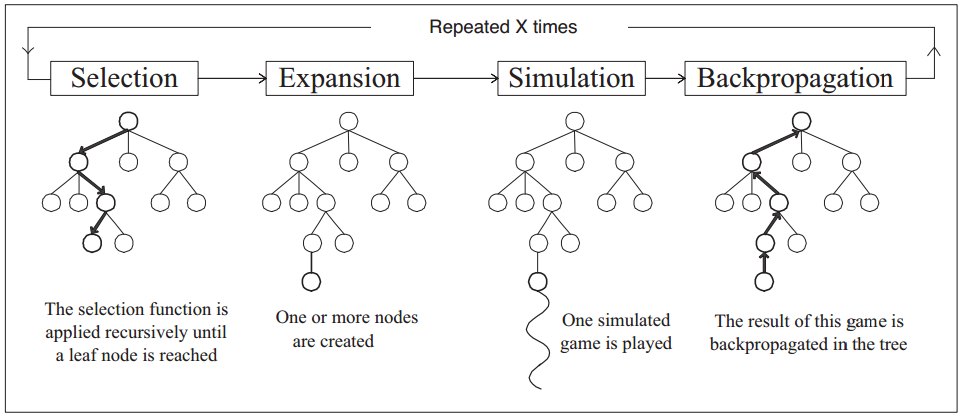
\includegraphics[width=\textwidth]{mcts}\\
		\centering
		\caption{Steps of the Monte-Carlo Tree Search, taken from Chaslot et al. \cite{MCTS_begin}.}
		\label{mcts}
	\end{figure}
	
	\subsubsection{The Use of Expanded Techniques with MCTS}
	Browne et al. \cite{survey} describes many different optimizations and enhancements to the basic MCTS and shows that there are many variants of MCTS which change different aspects of the four components of the algorithm.
	\\\\
	\noindent \textbf{Upper Confidence Bounds for Trees}\\\\
	\noindent Bandit based methods as used with MCTS are a modification of the selection phase of MCTS \cite{survey}. Browne et al. \cite{survey} describes bandit-based problems as a set of problems where there is an exploration-exploitation dilemma. This dilemma is that there is contention between the explorations of deeper variant moves with high win rate versus moves with few simulations associated with them (for the case of MCTS). Kocsis et al. \cite{bandit} applied a specific bandit algorithm for MCTS, known as UCB1. This application of a bandit-based policy for MCTS is known as the UCT algorithm. Here the algorithm uses random probabilities based on a policy mapping of what the next move that will be decided (as is generated in the expansion step). These generated moves are then checked against a regret (objective) function with the aim of minimizing the regret. The regret function used calculates the loss based on how many times the policies did not use the best possible path. The UCT algorithm, treats every child node of the move selection which has been explored as separate multi-armed bandit problems. The arms of each bandit problem are the available moves on the sub-tree and the child nodes are the weighted rewards of the paths calculated using the bandit-algorithm. During testing Kocsis et al. \cite{bandit} found that UCT appeared to produce a lower error than AB, MCTS and Monte-Carlo planning with minimax value update (A hybrid approach to tree search).\\
	
	\noindent James et al. \cite{wits} have however discovered that UCT operates far better when there is a preservation of the optimal decision rankings. This is very similar to what Edwards et al. \cite{AIM030} found with AB pruning. Caution must then be taken when using the UCT method as James et al. \cite{wits} found that if the distributions of the random simulations have small variances than UCT can become suboptimal and even worse than random. James et al. \cite{wits} noted that there has been a vast amount of work in researching alterations (such as UCT) in the selection and expansions steps of MCTS but less work has been done in the simulation step. 
	\\\\
	\noindent \textbf{Progressive Strategies for MCTS}\\\\
	\noindent Chaslot et al. \cite{progressive} suggested two progressive strategies which leave out infrequently visited nodes that can be selected and examined later. This is done using available information and some heuristics (which are computationally expensive) to select nodes which are visited often and invalidate the rest.\\
	
	\noindent Progressive bias as presented by Chaslot et al. \cite{progressive} and described in depth by Browne et al. \cite{survey} is a method which attempts to replace unreliable nodes (not visited often) with some heuristic function which takes in this suspect node as its input. This method works on the selection and expansion steps of MCTS. As the node is visited more (as the number of iterations of MCTS increases), the method will ensure that the heuristic's influence decreases. The heuristic may also only be applied after some fixed number of visits have passed for each node under question. This means that initially the MCTS functions as normal, after sometime the selection algorithm is applied to each node so the children with the highest heuristic values get chosen first due to there not being enough simulations to make an accurate prediction. As the number of simulations grows, the impact of both the heuristic function and the simulations are balanced. As the number of simulations keeps growing a boundary will be reached (determined by
	the heuristic function used) where the influence of the heuristic function will decrease until it has little effect whereas the effects of the simulated results now have a high impact on the outcome and the behaviour becomes similar to the basic approach of MCTS. \\
	
	\noindent Progressive unpruning is another method detailed by Chaslot et al. \cite{progressive} and described by Browne et al. \cite{survey} as a soft pruning method where possible decisions are ignored but may be evaluated later by using heuristic knowledge to reduce the size of the tree. This algorithm works when the number of simulations of some node equals a predefined threshold, a heuristic is then used to invalidate the less likely to be visited children nodes such that only the most likely nodes are selected. As the number of simulations gets bigger and further from the threshold, the children nodes should be progressively unpruned so that they may be evaluated. This reduces the number of sub-branches to deal with during the lower set of iterations of MCTS. Chaslot et al. \cite{progressive} has shown that this method helps with the time-complexity of the MCTS whilst improving the accuracy for a lower number of samples (simulations) when using MCTS. This provides the benefit that better results with lower error can be produced in a smaller time complexity than the vanilla MCTS.\\\\
	
	\noindent \textbf{Using Biasing Techniques with MCTS (Expert Knowledge)}\\\\
	Whitehouse et al. \cite{knowledge} proposed a method for initially biasing MCTS so that their commercial AI would seem more human to human players of their game. Their algorithm ISMCTS guesses potential game states and generates a game tree from the statistics of many potential game states by running simulations. Each iteration of the algorithm generates a new tree. They found that the injection of heuristic knowledge in MCTS was easier to implement than an expert heuristic system. They limited ISMCTS to only make decisions which can be contained in one round of their game because this algorithm is unable to look ahead to future rounds. The approach taken was to bias the initial selection step of MCTS and as the algorithm runs the applied bias tends to zero thereby avoiding the issue of weakening the AIs ability to take the best move for that round. The bias values are derived from existing knowledge. The tendency of the bias to go to zero is enforced during the backpropagation step when the updates of the node values which have a bias greater than 1 get their rewards increased whereas bias values less than 1 get reduced rewards. Whitehouse et al. \cite{knowledge} found that the MCTS chose the wrong move less than five percent from the tests conducted which was expected due to the random nature of the algorithm.\\
	
	\noindent There is however contention between Whitehouse et al. \cite{knowledge} and James et al. \cite{wits} as the former expects the injection of expert knowledge (bias) into MCTS will decrease the accuracy of the algorithm in choosing the most optimal decision whereas James et al. \cite{wits} found that the choice of bias is important in making sure that the performance of MCTS is not negatively affected and in some cases MCTS can perform better with bias added to the algorithm. There are some game problems where there is so little information supplied that running enough simulations to overcome this gap is infeasible - a solution here is to use an informed simulation. 
	
	\subsubsection{The Idea of Hybrid Tree Searches}
	Baier et al. \cite{hybrids} highlights that Minimax search techniques are very good at selecting the most optimal strategies but at the cost of performance whereas MCTS is very good at dealing with large and complex search domains (such as incomplete information) but at the cost of error - in some cases missing critical decisions which Minimax would not miss. Baier et al. \cite{hybrids} puts forward different areas of MCTS which can be modified to use the minimax search. The MCTS used in their experiments is the UCT form of the algorithm. A method which Baier et al. \cite{hybrids} described in the literature is to merge MCTS and Minimax is to use shallow (1-ply or 2-ply) searches at every simulation executed in MCTS - this however assumes the existence of an objective function and that the problem does not have incomplete knowledge.\\
	
	\noindent Baier et al. \cite{hybrids} goes on to describe three different approaches to merging MCTS and Minimax search, one in the simulation step of MCTS, another across the selection and expansion steps and a third in the backpropagation step of MCTS.
	\\\\
	\noindent \textbf{Minimax in the Simulation Step (MCTS-MR)}\\\\
	Rather than using uniformly random polices in the simulation step of MCTS rather Baier et al. \cite{hybrids} suggests Minimax searches of limited depth should be used to determine simulated decisions. However their method does not allow for objective functions so if Minimax cannot find a win or a loss than a random move must still be used. The power of this strategy is that certain errors which can occur when a random move is selected can be mitigated.
	\\\\
	\noindent \textbf{Minimax in the Selection and Expansion Steps (MCTS-MS)}\\\\
	Here Baier et al. \cite{hybrids} experimented in using Minimax searches at any node in the selection and expansions steps of MCTS which are determined by a given heuristic. Two heuristics suggested are to use a condition which checks the number of times a node has been visited, or use a threshold based on the loss of a certain path or a heuristic condition which will initiate a Minimax search if a simulation is found to be quick. A quick simulation suggests there is a terminal node close to the current node. This strategy can help with keeping unnecessary paths off the search tree whilst keeping nodes of importance (win-paths) in the tree.
	\\\\
	\noindent \noindent \textbf{Minimax in the Backpropagation Step (MCTS-MB)}\\\\
	Baier et al. \cite{hybrids} uses Minimax whenever the backpropagation step of MCTS has to switch from proven win/loss simulated returns to regular win/loss returns. This is caused when there are win states in child nodes whose parents are marked as a loss decision. Minimax is able to consider both terminal nodes and previous nodes (from previous MCTS iterations) which allows the algorithm to tell for which paths the opponent has a proven win. This strategy helps in making decisions be excluded more efficiently. A similar trick to MCTS-MS is to not use Minimax on sub-regions of the search domain where there are few terminal nodes (in the search tree).\\
	
	\noindent Baier et al. \cite{hybrids} found that MCTS-MS and MCTS-MB have a significant improvement in performance over the vanilla MCTS whereas MCTS-MR is not as flexible in terms of different search domains as the other two algorithms. 
	
	\subsubsection{Testing Methodologies}
	\label{testing}
	James et al. \cite{wits} defined domains specifically for their testing purposes. They used grid world and finite MDPs to produce less complex problems in which to conduct their experiments. They then ran the different algorithms and a basic random agent over these domains to get their results which they then took averages of by running thousands of the same experiment sets.  Whitehouse et al. \cite{knowledge} had a set domain in which they had to work with. Here testing was done using AI-versus-AI simulations and using a select number of real people to beta test different versions of their AI. Chaslot et al. \cite{progressive}, Browne et al. \cite{survey} and Kocsis et al. \cite{bandit} used many domains (2 or more) to run their experiments and to also see if the domain space itself could cause these different methods to behave differently.\\
	
	\subsection{Conclusion}
	Gwent poses an interesting problem due to the complexity of its domain by having incomplete information and a somewhat stochastic nature. Several AI tree search strategies will have to be tried to determine which will work best in this domain. The complexity of these methods creates a challenge on how to run tests and gain results. Due to nature of Gwent having sub-domain problems in its rule structure there is an expectation that a hybrid approach to MCTS and Minimax may offer good results - testing must be conducted to determine if this is true. Complex domains may confuse or bias results due to unforeseen problems inherent in those complexities and so a limited and constrained sub-domain of the problem should be chosen in order to ensure that the hypothesis is able to be fairly tested and an experimental method which is sound is implemented.
	
	\section{Research Methodology}
	\subsection{Introduction}
	The proposed methodology attempts to uses similar strategies as seen in the literature under section \ref{testing}. An example is using AI-versus-AI simulations to find which AIs perform better than other AIs.
	
	\subsection{Hypothesis}
	My hypothesis states that:\\
	\indent\textbf{A hybrid MCTS and Minimax method will outperform in time complexity and win rate against the independent methods when applied to the game of Gwent.}\\\
	
	\noindent The null hypothesis is therefore that there would be no difference in the performance of a hybrid MCTS method and the standalone algorithms in terms of time complexity and win rate when applied to the game of Gwent. The overall research will attempt to find which theoretical outcome is true.
	
	\subsubsection{Motivation}
	Gwent is an interesting domain as it is disjoint. Depending on the rule set there are many sub-domains to search when dealing with some of the special rules - an example is the medic ability described in section \ref{background}. MCTS methods are very good at dealing with large domains which are intractable to search by running many simulations on the domain but the main drawback is that these methods do not select the most optimal move - rather a simulated move which is a good approximate optimal from the sample space \cite{survey}. Minimax on the other hand does not handle large and intractable domains as well because the approximations that have to be made to get the AI to work in an acceptable time are very harsh. Minimax however is very good at selecting the best set of strategies when it can search the entire domain or a large enough sample of a domain \cite{AIModern}. This implies that these methods work on the different trade-offs of AI tree search methods which are resource complexity versus confidence in making the best decision. A hybrid approach attempts to bridge these two apposed methods together to try and take the benefits of both methods whilst avoiding their drawbacks \cite{hybrids}. The disjoint nature of Gwent means that on top of applying a hybrid directly, an AI which uses MCTS with modifications for the overall domain and a condition which allows the AI to use minimax to deal with the sub-domains which may appear either in simulation or after the move has been selected. If the sub-move set happens to become very large MCTS can be applied over minimax. This is an easy check to make by using basic statistics on the current collections of cards. 
	
	\subsection{Restrictions Placed on the Domain}
	A sub domain of Gwent must be chosen in order to limit the scope of this research so that it will be feasible in the allotted time-frame. The chosen decks will be limited to two decks which have cards chosen so that the decks have similar attributes. These decks must keep some of the special rules of the game such as being able to revive discarded cards but will not contain cards which can target specific opponent cards as these two special abilities are very similar in terms of the problem they present to an AI. The leader cards and their abilities will also be ignored. All AI (player) responses will be limited to 50ms response time as this ensures that the many experimental games that need to be run can be done in a realistic time-frame.
	
	\subsection{Experimental Method}
	This research requires a large amount of programming and empirical analysis. The first task is to build a game supervisor which produces the domain and enforces the rules of the game for the AIs to have a framework to use. Several AIs using versions of MCTS and minimax also need to be made. A random AI agent who plays a random move from a valid move list (for that game state) must also be produced. Then a hybrid AI needs to be constructed. A small tool will also be built to compute the statistics from the results generated. Finally a visualizer will be made which will be able to show AIs playing each other and also allow a human to play an AI - this will be done for demonstration purposes.\\\\
	All the AIs must be run against the random agent to determine if they perform better than random on the domain. A tournament setting will then be setup where different AIs will be pitted against each other in a round-robin style to find which algorithms perform the best. This will be done in rounds of experiments where AI opponents will be set so that a large enough set of results can be collected and analysed to determine which AIs are better for each group of experimental rounds. Each individual experiment in a round will pit the same two AIs but the game state that is set will be randomly generated based on the available cards. The player who is chosen to go first will not be chosen at random but rather both AIs for any given set of rounds will each start fifty percent of that batch of experiments. The number of runs will be in the region of thousands of runs, this is based on the sourced literature under section \ref{testing}. The actual number of final runs used will be determined by how quickly a game can be run. An average of the results will then be taken and other statistics such as variance will also be tracked. The top AI will then be validated by playing a small limited number of games against a human to ensure that the system is working correctly. Another check will be to run the top AI against itself in its own set of experiments in order to analyse what happens. 
	
	\subsection{Implementation}
	The programming for the game supervisor and all the AI methods will be done in C++. As described by Bronson et al. \cite{bronson2012c++} C++ allows for the use of inheritance techniques which allows for concepts such as the base tree implementations to be shared between the different AI implementations. C++ is also a compiled language which provides lower level access to a computer systems resources which will allow me to make code which will run faster than equivalent code which runs in an interpreted languages virtual environment. Another useful implication of using C++ is that many advanced parallel computing libraries such as OpenMP are extensions of C and C++ \cite{parallel}. This allows me to modify code to make it parallel if problems with time and space complexity arise during development of this experimental framework. All results generated will be stored as files on secondary storage medium to be processed later and kept so that any problems that may arise due to programming errors can be analysed and fixed. The visualizer will also be built using C++ and the SDL library for the graphical output.\\\
	
	\noindent All the AI implementations will make use of some parts of the game supervisor such as building game states and enforcing rules which will then be used to simulate different decisions in the respective AIs.  
	
	\subsection{Conclusion}
	Gwent is an interesting domain to apply these techniques to because it is disjoint. This provides an opportunity to experiment with different tree search methods in order to analyse their behaviours and respective performance. The domain does have to be limited to make the domain easier for the AIs to handle. C++ is a good choice in programming language to implement this experimental framework because it provides lots of control to the programmer and has well documented and industry standard libraries for parallelisation. The AIs will be tested by performing AI-versus-AI simulations and collecting the statistics of thousands of simulations. A small limited amount of human-versus-AI plays will also be used to validate that the respective AIs are working as intended. The presented plan will breakdown the required parts needed to build the experimental framework and then fit these deliverables into the time available for this project.
	
	\section{Research Plan}
	\subsection{Introduction}
	This research project is fairly large with many components which need to be built before any results can be generated. This creates some risk in terms of delivering usable results and completing the research in the available time. A strong list of success measures is therefore needed to help at the end of the research project to determine whether the aim has been achieved.
	
	\subsection{Risks}
	
	\begin{itemize}
		\item The greatest risk is that The runs of any experiment may take too much time to execute which may lead to completing the analysis of the AIs becoming impossible to perform with the given time constraints. Some solutions would be to reduce the number of AIs, the scale of the domain, the number of experiments run per round or make the time and space limits of the respective AIs smaller. Another solution would be to apply high performance computing (HPC) techniques to the problem.
		
		\item The AIs may be too difficult to implement within the current time constraints. A solution to this risk would be to scale the research down to a smaller sub-problem and work from there. An example would be to compare MCTS and minimax and leave out the hybrid approach.
		
		\item The chosen domain and AI implementations are stochastic in nature. This means that it is possible that the AIs may choose a random action that is always bad and therefore skew the results generated based on this bad sample of the choices that can be made. A solution would be to modify the AIs to make use of some progressive strategies which make use of some bias in the chosen moves, so that more ideal moves are chosen based on past experience \cite{progressive}.
		
	\end{itemize}
	
	\subsection{Deliverables}
	\begin{itemize}
		\item A game supervisor or environment which programmatically models the domain
		\item A Random agent
		\item An AI which implements a MCTS method 
		\item An AI which implements a minimax method
		\item An AI which implements a Hybrid method
		\item A Result processing tool
		\item A Visualizer to be able to demo the experimental system
		\item The final Report
	\end{itemize}
	
	\subsection{Measures of Success}
	\begin{itemize}
		\item An AI has been found to perform better than other AIs tested.
		\item The AIs have been compared to each other
		\item The AIS perform better than the random agent.
		\item The rules of Gwent have been successfully programmed into a game supervisor.
		\item At least three AIs which are different have been produced.
	\end{itemize}
	
	\subsection{Time Plan}
	% \begin{tabular}{|l|l|l|p{5cm}|p{5cm}|p{5cm}|}
	% \caption{Research Time Plan}
	% \label{time-plan}
	
	\begin{table}[H]
		\centering
		\resizebox{\textwidth}{!}{
			\begin{tabular}{|l|l|l|p{6cm}|p{6cm}|p{6cm}|}
				\hline
				\textbf{Week} & \textbf{Date} & \textbf{Interest} & \textbf{Research Task} & \textbf{Motivation} & \textbf{Period} \\ \hline
				\textbf{1} & 15th May & ACML Test and HPC Project & N/A & Need to complete course work. & Block 2 \\ \hline
				\textbf{2} & 22nd May & ACML Project and DIP Exam & N/A & Exams begin. & Exams \\ \hline
				\textbf{3} & 29th May & ACML Exam & N/A & June Exams. & Exams \\ \hline
				\textbf{4} & 5th Jun & DIP Exam & N/A & June Exams. & Exams \\ \hline
				\textbf{5} & 12th Jun &  & N/A & Final June exam in a week. Have a week to study for it. & Exams \\ \hline
				\textbf{6} & 19th Jun & HPC Exam & Begin programming game supervisor & Begin most important component. HPC Exam on 19th June so have the rest of the week. & Exams \\ \hline
				\textbf{7} & 26th Jun &  & Finish game supervisor & The supervisor and game rules have to be implemented before an AI development can be done. & Break \\ \hline
				\textbf{8} & 3rd Jul &  & Develop the random agent AI & This should be a fairly simple program because it takes the list of available moves provided by the game supervisor and chooses a random one to play. & Break \\ \hline
				\textbf{9} & 10th Jul & Birthday & Begin development of standard MCTS AI & MCTS is the easiest implementation of the three major types of AI tree search algorithms being investigated. & Break \\ \hline
				\textbf{10} & 17th Jul &  & Finish development of MCTS AI & All tree AI algorithms have underlying structure and method which are similar. The first AI will take longer to implement correctly and sucessive AIs will be easier to make as problems are discovered and solved. & Break \\ \hline
				\textbf{11} & 24th Jul &  & Start development on Minimax AI & The Hybrid AI can only be built once both the individual AIs are built. & Block 3 \\ \hline
				\textbf{12} & 31st Jul &  & Finish development of Minimax AI & This AI should be quicker to develop than previous AIs. & Block 3 \\ \hline
				\textbf{13} & 7th Aug &  & Start development of Hybrid AI & This is the most critical development phase as this is the heart of the research. & Block 3 \\ \hline
				\textbf{14} & 14th Aug &  & Finish development of the Hybrid AI & This must be complete before analysis of the research can take place. & Block 3 \\ \hline
				\textbf{15} & 21st Aug &  & Run experimental tests using AIs and collect data & These tests will be lengthy as large enough sample data must be collected before accurate results can be found. & Block 3 \\ \hline
				\textbf{16} & 28th Aug &  & Run experimental tests using AIs and collect data & Continued tests as these experiments may take days to run. & Block 3 \\ \hline
				\textbf{17} & 4th Sep &  & Run experimental tests using AIs and collect data & An extra week to validate and tweak any experiments which may not be producing sane results. & Block 3 \\ \hline
				\textbf{18} & 11th Sep &  & Interpret results and begin to write report. & The report will take a few weeks to write. & Vacation \\ \hline
				\textbf{19} & 18th Sep &  & Continue to write report & Depending on the results the difficulty in interpretation may be different. & Block 4 \\ \hline
				\textbf{20} & 25th Sep &  & Finish report & The report should be finished a few weeks early. & Block 4 \\ \hline
				\textbf{21} & 2nd Oct & Away over weekend & Extra time for research & Extra time allocated in case something goes wrong or for supervisor to provide feedback. & Block 4 \\ \hline
				\textbf{22} & 9th Oct &  & Extra time for research & Extra time allocated in case something goes wrong or for supervisor to provide feedback. & Block 4 \\ \hline
				\textbf{23} & 16th Oct &  & Research Project Should be complete & Middle of October is when the project should be completed. & Block 4 \\ \hline
				\textbf{24} & 23rd Oct &  &  &  & Block 4 \\ \hline
				\textbf{25} & 30th Oct & Report submission &  & The submission of final documentation is the beginning of November. & Block 4 \\ \hline
			\end{tabular}
		}
		\caption{Research Time Plan}
		\label{time-plan}
	\end{table}
	
	\subsection{Conclusion}
	Gwent is an unknown domain in terms of how these variant types of tree search algorithms may perform. This means that many roadblocks may appear such as the experimental runs may take too long for the amount of time available to complete the research project. Several solutions exist such as reducing the scope of the research, and applying HPC techniques to the implementation in order to speed up the overall system. There are many components required to complete this project and a strong list of success measures therefore exists to help determine whether the aim has been achieved at the end of the research.
	
	\section{Conclusion}
	Gwent is an exciting domain for artificial intelligence because it has disjoint sub-domains and a stochastic nature. This provides an opportunity to experiment with different tree search methods in order to analyse their behaviours and respective performance. The aim of this research is to compare MCTS and minimax methods when applying them to Gwent and then produce a hybrid AI of the two types of methods to determine if a hybrid approach performs better in time complexity and win rate. The domain must be restricted in order to constrain the research project to make it viable. The cards used will be pre-chosen, the leader cards ability will be ignored, special rules which target the opposing player's cards will be removed and the AI decision time limit will be set to 50ms. These AI implementations will be developed in C++ and will be analysed by using AI-versus-AI simulations in a tournament style experiment. Each round of the tournament will contain thousands of experiments where the game states are randomly generated. There are risks with this proposed research such as the experimental runs taking too long for the amount of time available to complete the research project. This can be solved by reducing the scope of the research, and applying HPC techniques to the implementation in order to speed up the overall system. The main indication that this project is successful is if the implemented AIs are compared to each other on the domain and one is found to be better than the others whilst not performing worse than the random agent. The research is interesting because Gwent has not had these algorithms applied to it in any research environment due to the game being so new. This domain also provides difficulties that may cause interesting results with these methods such as computational performance problems.
	
	\break
	%\begin{appendices}
	%\appendixpage
	%\noappendicestocpagenum
	% \addappheadtotoc
	
	\section*{Glossary of Terms}
	\setlist{nosep}
	\begin{myitemize}
		\item[] \itab{\textbf{AB}} 			\quad\quad\tab{-} \tab{Alpha-Beta}\\
		\item[] \itab{\textbf{AI}} 			\quad\quad\tab{-} \tab{Artificial Intelligence}\\
		\item[] \itab{\textbf{ACML}} 		\quad\quad\tab{-} \tab{Adaptive Computation and Machine Learning}\\
		\item[] \itab{\textbf{DIP}} 		\quad\quad\tab{-} \tab{Digital Image Processing}\\
		\item[] \itab{\textbf{HPC}} 		\quad\quad\tab{-} \tab{High Performance Computing}\\
		\item[] \itab{\textbf{ISMCTS}} 		\quad\quad\tab{-} \tab{Information Set Monte-Carlo Tree Search}\\
		\item[] \itab{\textbf{MCS}} 		\quad\quad\tab{-} \tab{Monte-Carlo Simulation}\\
		\item[] \itab{\textbf{MCTS}} 		\quad\quad\tab{-} \tab{Monte-Carlo Tree Search}\\
		\item[] \itab{\textbf{MCTS-MB}} 	\quad\quad\tab{-} \tab{MCTS with Minimax Backpropagation}\\
		\item[] \itab{\textbf{MCTS-MR}} 	\quad\quad\tab{-} \tab{MCTS with Minimax Rollouts}\\
		\item[] \itab{\textbf{MCTS-MS}} 	\quad\quad\tab{-} \tab{MCTS with Minimax Selection}\\
		\item[] \itab{\textbf{MDP}} 		\quad\quad\tab{-} \tab{Markov Decision Processes}\\
		\item[] \itab{\textbf{UCB}} 		\quad\quad\tab{-} \tab{Upper Confidence Bounds}\\
		\item[] \itab{\textbf{UCT}} 		\quad\quad\tab{-} \tab{Upper Confidence Bounds for Trees}\\
	\end{myitemize}
	
	%\end{appendices}
	\break
	\bibliographystyle{plain}
	\bibliography{biblist}{}
	
\end{document}\grid
